\documentclass[a4paper,10pt]{article}

\usepackage{graphicx}
\usepackage[ansinew]{inputenc}
\usepackage[spanish]{babel}
\usepackage{hyperref}
\usepackage{listings}
\usepackage{mips}
\usepackage{verbatim}
\usepackage{pdfpages}

\title{		\textbf{Versi�n en C del comando rev }}

\author{	Lucas Simonelli, \textit{Padr�n Nro. 93111}                     \\
            \texttt{ lucasp.simonelli@gmail.com }                                              \\[2.5ex]
            Tom�s Boccardo, \textit{Padr�n Nro. 00.000}                     \\
            \texttt{ direcci�n de e-mail }                                              \\[2.5ex]
            Andr�s Sanabria, \textit{Padr�n Nro. 00.000}                     \\
            \texttt{ direcci�n de e-mail }                                              \\[2.5ex]
            \normalsize{2do. Cuatrimestre de 2013}                                      \\
            \normalsize{66.20 Organizaci�n de Computadoras  $-$ Pr�ctica Martes}  \\
            \normalsize{Facultad de Ingenier�a, Universidad de Buenos Aires}            \\
       }
\date{}

\begin{document}

\maketitle
\thispagestyle{empty}   % quita el n�mero en la primer p�gina


%\begin{abstract}
%Este art�culo es un modelo que proporciona a los alumnos las instrucciones necesarias para preparar sus informes para la asignatura \textit{66.20 Organizaci�n de %Computadoras} (pr�ctica Viernes). El informe podr� contener (optativo) un resumen de no m�s de 150 palabras. La primera p�gina del art�culo deber� seguir el formato que se ilustra en el presente modelo y deber� contener el t�tulo, los nombres de los autores, sus n�meros de padr�n, sus direcciones de e-mail, y el resumen (si tuviese). La primera p�gina del informe no debe ser numerada.
%\end{abstract}

\newpage
\section{Introducci�n}

En el presente trabajo pr�ctico se elabor� una versi�n en C del comando \textit{rev} de Unix\footnote{\url{http://linux.about.com/library/cmd/blcmdl_rev.htm}}, que
puede ejecutarse sin problemas tanto en linux sobre x86 como en netBSD sobre MIPS32.


\section{Funci�n}
El ejecutable tendr� el mismo objeto que el comando rev, es decir, leer� un archivo por alguno de los canales ofrecidos y lo invertir� l�nea a l�nea.


\section{Comandos para la compilacion}
Para compilar el programa, deber� introducirse el siguiente comando:
\begin{verbatim}
#compilamos
~$gcc -o tp0 main.c

#corremos
~$./tp0 [archivo]
\end{verbatim}

\subsection{Sintaxis de uso}
\begin{verbatim}
$ ./tp0 -h
Usage:
./tp0 -h
./tp0 -V
./tp0 [file...]
Options:
-V, --version, print version and quit.
-h, --help, print this information and quit.

Examples:
./tp0 foo.txt bar.txt
./tp0 gz.txt
echo "Hola mundo" | ./tp0
\end{verbatim}

\section{Corridas de prueba}
(Los archivos se facilitan junto con este informe en la entrega digital)
\subsection{Corrida con archivo de par�metro}
\begin{verbatim}
~$./tp0 ejemplo.txt
1elif ed aenil aremirp al se atsE
.adnuges al se atse y

\end{verbatim}
\subsection{Corrida con entrada de stdin}
\begin{verbatim}
~$echo "Hola mundo" | ./tp0
odnum aloH
\end{verbatim}

\section{C�digo fuente}
\lstinputlisting[language=C]{../main.c}

\section{C�digo MIPS32}
\lstset{language=[mips]Assembler}
\lstinputlisting{../fuente.mips}

\section{Conclusiones}

Se aprendieron las generalidades del uso de gxemule.

\section{Enunciado}
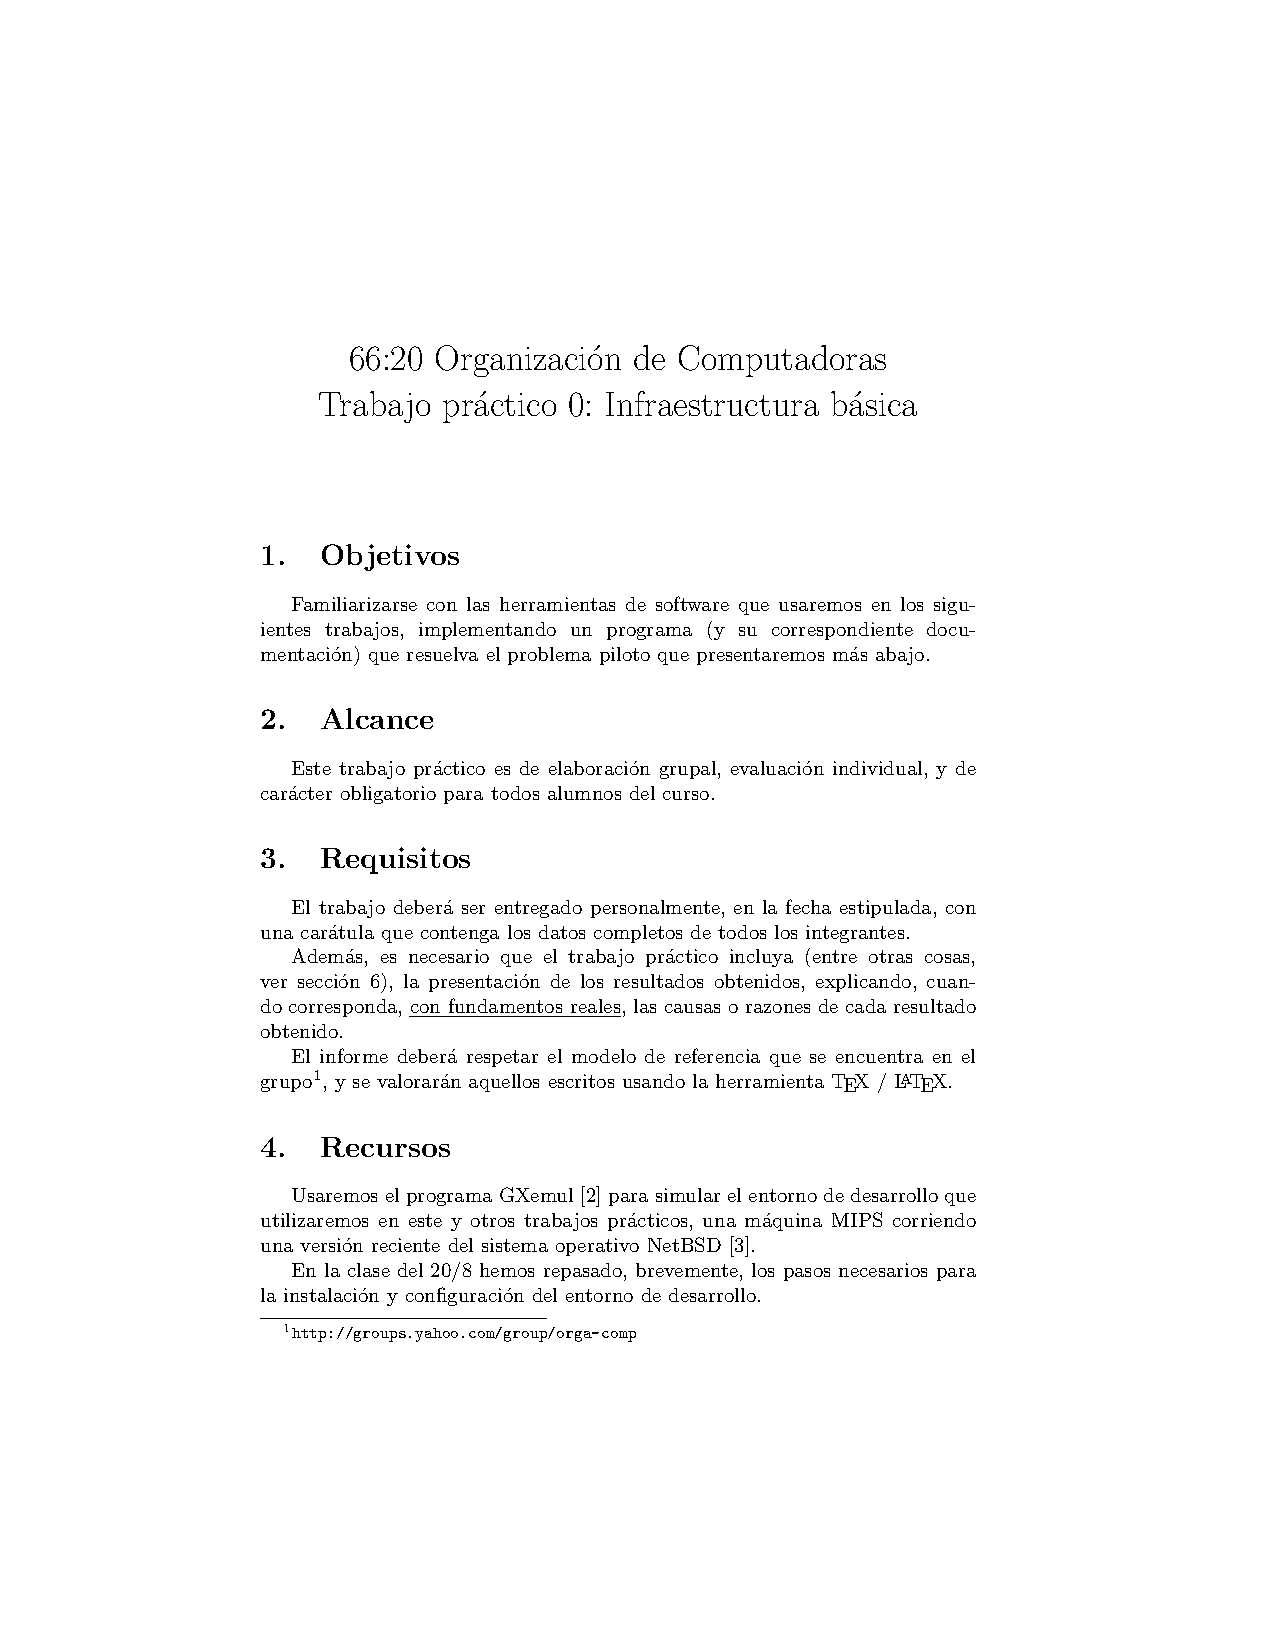
\includepdf[scale=0.8,pages={1,2,3,4}]{../enunciado.pdf}

\begin{comment}
\begin{thebibliography}{99}

\bibitem{INT06} Intel Technology \& Research, ``Hyper-Threading Technology,'' 2006, http://www.intel.com/technology/hyperthread/.

\bibitem{HEN00} J. L. Hennessy and D. A. Patterson, ``Computer Architecture. A Quantitative
Approach,'' 3ra Edici�n, Morgan Kaufmann Publishers, 2000.

\bibitem{LAR92} J. Larus and T. Ball, ``Rewriting Executable Files to Mesure Program Behavior,'' Tech. Report 1083, Univ. of Wisconsin, 1992.

\end{thebibliography}
\end{comment}
\end{document}
